%%%%%%%%%%%%%%%%%%%%%%%%%%%%%%%%%%%%%%%%%
% Journal Article
% LaTeX Template
% Version 2.0 (February 7, 2023)
%
% This template originates from:
% https://www.LaTeXTemplates.com
%
% Author:
% Vel (vel@latextemplates.com)
%
% License:
% CC BY-NC-SA 4.0 (https://creativecommons.org/licenses/by-nc-sa/4.0/)
%
% NOTE: The bibliography needs to be compiled using the biber engine.
%
%%%%%%%%%%%%%%%%%%%%%%%%%%%%%%%%%%%%%%%%%

%----------------------------------------------------------------------------------------
%	PACKAGES AND OTHER DOCUMENT CONFIGURATIONS
%----------------------------------------------------------------------------------------

\documentclass[
	a4paper, % Paper size, use either a4paper or letterpaper
	10pt, % Default font size, can also use 11pt or 12pt, although this is not recommended
	unnumberedsections, % Comment to enable section numbering
	twoside, % Two side traditional mode where headers and footers change between odd and even pages, comment this option to make them fixed
]{LTJournalArticle}

\addbibresource{bibliography.bib} % BibLaTeX bibliography file

\runninghead{Jak získat energii z černé díry?} % A shortened article title to appear in the running head, leave this command empty for no running head

% \footertext{\textit{Journal of Biological Sampling} (2024) 12:533-684} % Text to appear in the footer, leave this command empty for no footer text

\setcounter{page}{1} % The page number of the first page, set this to a higher number if the article is to be part of an issue or larger work

%----------------------------------------------------------------------------------------
%	TITLE SECTION
%----------------------------------------------------------------------------------------

\title{Jak získat energii z černé díry?} % Article title, use manual lines breaks (\\) to beautify the layout

% Authors are listed in a comma-separated list with superscript numbers indicating affiliations
% \thanks{} is used for any text that should be placed in a footnote on the first page, such as the corresponding author's email, journal acceptance dates, a copyright/license notice, keywords, etc
\author{%
	Artem Gorodilov\textsuperscript{1}
}

% Affiliations are output in the \date{} command
\date{\footnotesize\textsuperscript{\textbf{1}}Ústav teoretické fyziky a astrofyziky, Prírodovedecka fakulta, Masarykova univerzita}

% Full-width abstract
\renewcommand{\maketitlehookd}{%
	\begin{abstract}
		\noindent Tento článek se zabývá potenciálním zdrojem energie pro vyspělé mimozemské civilizace, zejména ty, které jsou klasifikovány jako typ III na Kardaševově stupnici. Primárně se zaměřuje na fyzikálně podložený přístup: využití energie z BH. Studie pojednává o modelu získávání energie z BH zvaném Penroseův stroj v rámci obecné teorie relativity. Výsledky naznačují, že BH by mohla sloužit jako výkonný a udržitelný zdroj energie pro civilizace, které se snaží rozšířit svůj vliv napříč galaxiemi.
	\end{abstract}
}

%----------------------------------------------------------------------------------------

\begin{document}

\maketitle % Output the title section

%----------------------------------------------------------------------------------------
%	ARTICLE CONTENTS
%----------------------------------------------------------------------------------------

\section{Úvod}

Jak lze uspořádat ekonomiku mimozemských civilizací, aby získávaly energii na dobývání nových a nových galaxií? Můžeme spekulovat o tachyonových generátorech, konvertorech energie z vesmírů s odlišnou fyzikou nebo o velké peci spalující temnou hmotu. Pokud však k otázce přistoupíme realističtěji, aniž bychom vymýšleli zcela exotické entity, budeme muset každou hvězdu stočit do Dysonovy sféry \autocite{dyson1960}? Ve skutečnosti existuje tak účinný mechanismus výroby energie, který by byl hoden civilizace úrovně 3 na stupnici Kardasheva \autocite{kardashev1964}. A zrojem této energie by byla černá díra (ČD)

%------------------------------------------------

\section{Fyzika černých děr}

\subsection{Statická nerotující černá díra}

Skutečnou ČD se zatím nikomu nepodařilo vytvořit v experimentálním zařízení na Zemi. Proto hovoříme o jejich modelování na základě Obecné Teorie Relativity (OTR). Existují různé modely. První a nejjednodušší z nich se objevil téměř ihned po Einsteinově zveřejnění OTR v letech 1915-1916 a jeho autorem je německý fyzik Karl Schwarzschild. Ten se rychle chopil matematického aparátu nové teorie a rychle našel první přesné řešení Einsteinových rovnic \autocite{schwarzschild1999}. 

Řešením byla nejjednodušší, nerotující a beznábojová ČD. Tedy nějaká oblast, v níž je prostor deformován do té míry, že únik z ní by vyžadoval nadsvětelnou rychlost. Hranice této oblasti se nazývá horizont událostí a je definována Schwarzschildovým poloměrem:

\begin{equation*}
	r_s = \frac{2GM}{c^2}
\end{equation*}

Schwarzschildovu metriku pro nerotující nenabitou ČD ve standardních Schwarzschildových souřadnicích $(t, r, \theta, \phi)$ ukazuje rovnice (\ref{eq:swarz_metric}). Prvek přímky je uveden v rovnici (\ref{eq:line_element}).

\begin{equation}
g_{\mu\nu} =
\begin{bmatrix}
	-\left(1 - \frac{2GM}{r}\right) & 0 & 0 & 0 \\
	0 & \left(1 - \frac{2GM}{r}\right)^{-1} & 0 & 0 \\
	0 & 0 & r^2 & 0 \\
	0 & 0 & 0 & r^2 \sin^2 \theta
	\label{eq:swarz_metric}
\end{bmatrix}
\end{equation}

\begin{equation}
	\begin{split}
		ds^2 &= -\left( 1 - \frac{2GM}{r} \right) dt^2 
		+ \left( 1 - \frac{2GM}{r} \right)^{-1} dr^2 \\
		&\quad + r^2 d\theta^2 
		+ r^2 \sin^2 \theta d\phi^2
	\end{split}
	\label{eq:line_element}
\end{equation}

Později se ukázalo, že ČD není jen matematická hračka. Když se masivní hvězda po spotřebování vodíku zhroutí a exploduje v supernově. Při určité kombinaci počáteční hmotnosti hvězdy a hmotnosti zbytku po výbuchu supernovy (viz tabulka (\ref{tab:masses})). se komprese hvězdy nemůže zastavit a podle všeho by se měla celá nacházet v samotném středu ČD, v místě, kde by teoreticky měla být nekonečná hustota a nekonečné zakřivení prostoru a času. Takovému bodu se říká singularita. Ukazuje se, že horizont událostí je jakousi podmíněnou hranicí černé díry. Poloměr, při kterém je úniková rychlost rovna rychlosti světla.

\begin{table*} % Single column table
    \caption{Vývoj hvězd podle jejich hmotnosti}
    \centering
    \begin{tabular}{l l r}
        \toprule
        Počáteční hmotnost hvězdy $[\textup{M}_\odot]$ & Hmotnost zbytku (jádra) $[\textup{M}_\odot]$ & Konečné stádium \\
        \midrule
        $< 8$  & ---  & Bílý trpaslík \\
        $8 - 20$  & $1.4 - 3$ & Neutronová hvězda \\
        $20 - 40$  & $> 3$ & Černá díra \\
        $> 40$ & Úplný kolaps & Černá díra (přímý kolaps) \\
        \bottomrule
    \end{tabular}
    \label{tab:masses}
\end{table*}


\subsection{Nestatická rotující černá díra}

Schwarzschildova ČD je přitom poněkud zjednodušený model. S největší pravděpodobností ve vesmíru žádné takové ideální ČD neexistují. A důvodem je rotace hvězd. Slunce vykoná úplnou otáčku kolem své osy přibližně za $25.67 \text{d}$ (na rovníku). Hmotnější hvězdy rotují ještě rychleji a právě hmotné hvězdy jsou kandidáty na roli budoucích černých děr. Když se tyto hvězdy zhroutí, jejich rychlost rotace se mnohonásobně zvýší. To je důsledek zákona zachování hybnosti. Například: kdyby se Slunce smrsklo na svůj Schwarzschildův poloměr $\approx 3 \text{km}$, přičemž by si plně zachovalo svůj točivý moment, otáčelo by se rychlostí až 1000 otáček za sekundu a rychlost na rovníku by činila asi 45\% rychlosti světla.  

Ukazuje se, že ČD vzniklé při kolapsu hvězd by měly rotovat, a to poměrně rychle. Co přesně se ale v ČD otáčí? Vždyť mluvíme o nekonečně malém bodě v prostoru, co s tím má společného rotace? ČD je popsána pouze třemi parametry: hmotností, hybností a elektrickým nábojem. Hybnost je právě zodpovědná za rotaci a podle zákona zachování energie - všechny tyto veličiny se musí zachovat, takže ČD musí zdědit hybnost od mateřské hvězdy. 

Řešení rovnic OTR se podařilo získat až téměř 50 let po Schwarzschildově úspěchu. Podařilo se to v roce 1963 Royi Kerrovi \autocite{kerr1963}. Kerrovu metriku v Boyerových-Lindquistových souřadnicích $(t, r, \theta, \phi)$ představuje vzorec (\ref{eq:kerr_metric}).

\begin{equation}
	\begin{split}
		ds^2 &= -\left( 1 - \frac{2GM r}{\Sigma} \right) dt^2 
		- \frac{4GM a r \sin^2\theta}{\Sigma} dt d\phi 
		+ \frac{\Sigma}{\Delta} dr^2 \\
		&+ \Sigma d\theta^2 \quad + \left( r^2 + a^2 + \frac{2GM a^2 r \sin^2\theta}{\Sigma} \right) \sin^2\theta d\phi^2
	\end{split}
	\label{eq:kerr_metric}
\end{equation}

kde

\begin{equation*}
	\Sigma = r^2 + a^2 \cos^2\theta, \quad
	\Delta = r^2 - 2GM r + a^2.
\end{equation*}

Rotace ČD činí matematiku pro výpočet mnohem složitější a fyzika rotující ČD se stává mnohem rozmanitější. Již v době Schwarzschilda byl v OTR znám jeden jev související s rotací těles. Prvním pozorovacím potvrzením teorie byla precese dráhy Merkuru. Perhelium Merkuru se neustále posouvalo. To se obvykle přisuzuje gravitačnímu vlivu jiných nebeských těles. Astronomové se dokonce pokusili hledat planetu uvnitř Merkurovy dráhy a pojmenovali ji Vulkán \autocite{weinstein2014}. Řešení však našel až Einstein v roce 1915 jako součást OTR. Ukázalo se, že podle OTR rotující tělesa unášejí prostor a ten se podobně jako vír stáčí ve směru rotace tělesa. Tento jev se nazývá Lense-Thirringův efekt \autocite{pfister2007}. Vizuální znázornění je uvedeno na obrázku (\ref{fig:lense-thirring}).

\begin{figure} % Single column figure
	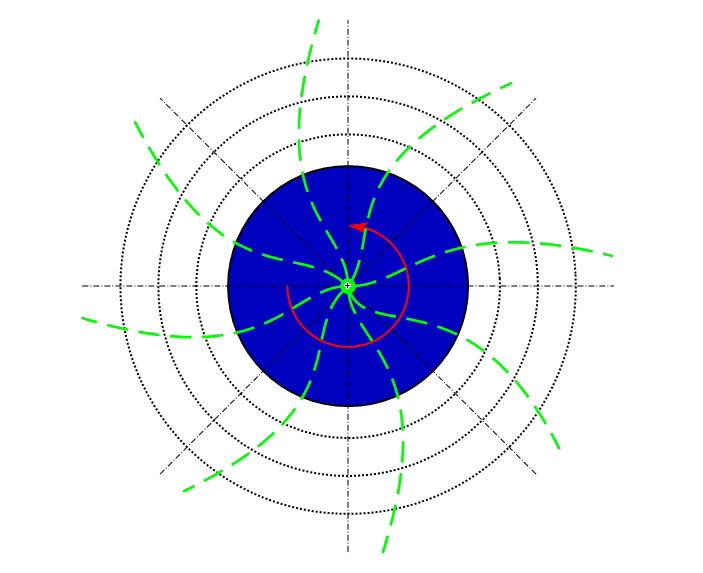
\includegraphics[width=\linewidth]{lense-thirring.png}
	\caption{Diagram of Frame-dragging effect. Source: \textcite{zhang2024}.}
	\label{fig:lense-thirring}
\end{figure}

Statické ČD jsou sféricky symetrické. Rotující objekty jsou naopak v rovníkové oblasti roztažené. Tomuto efektu podléhá i horizont událostí (HU) rotující ČD, který se podobá rotačnímu elipsoidu. Taková ČD musí mít ještě jednu důležitou plochu, která se nazývá statická limita. Je to hranice prostoru, uvnitř které těleso nemůže zůstat pro vnějšího pozorovatele v klidovém stavu. V této oblasti se těleso nevyhnutelně stočí do víru časoprostoru v napětí rotace ČD. V nerotující ČD se HU a limita statičnosti shodují. V rotující ČD se dotýkají na pólech. Oblast mezi statickou limitou a HU se nazývá ergosféra (viz obrázek (\ref{fig:ergosphere})). 

\begin{figure} % Single column figure
	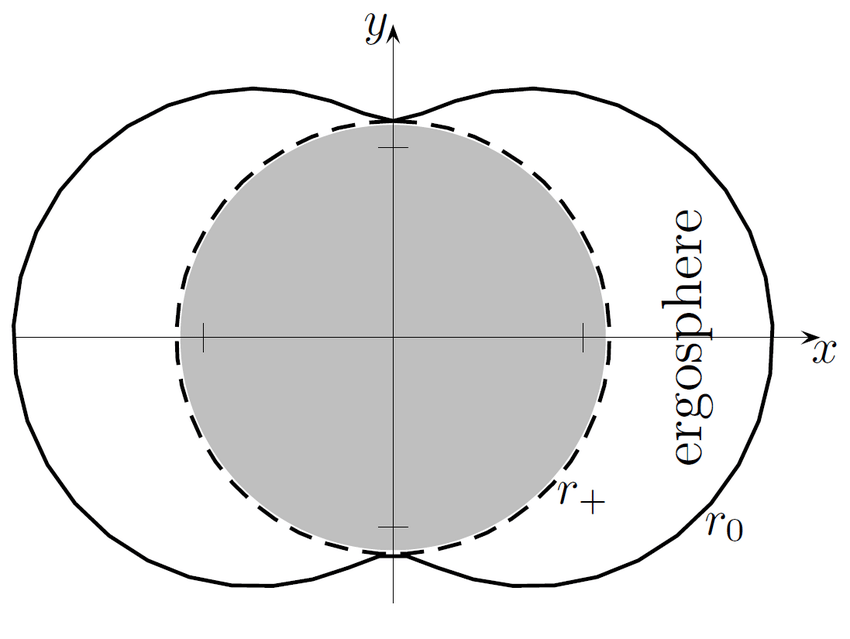
\includegraphics[width=\linewidth]{ergosphere.png}
	\caption{Event horizon $r_+$ and ergosphere $r_0$ of a rotating Kerr Black Hole. Source: \textcite{scharpf2017}.}
	\label{fig:ergosphere}
\end{figure}

\section{Penroseův stroj}

Jakmile se dostanete za HU, není cesty ven. Je však zcela reálné dostat se do ergosféry a vrátit se zpět. V tomto smyslu funguje jako kolotoč: pokud se k němu připojíte a pak se od něj včas odpojíte, můžete získat dodatečnou energii díky rotaci přenesením točivého momentu rotace. Současně se zpomaluje i samotná ČD. A to je právě ten princip získávání energie. 

V roce 1969 popsal matematik Roger Penrose zajímavou vlastnost Kerrovy ČD \autocite{penrose2002}. Ukázalo se, že k opuštění ergosféry není nutné na ni působit obrovskou energií. Stačí správně použít zákon zachování hybnosti. Představme si, že nějaké těleso, které dopadne do ergosféry, se tam rozpadne na dvě části: jedna část spadne pod HU a je pohlcena ČD a druhá část se podle zákona zachování hybnosti odrazí zpět a vyletí z nejbližšího okolí ČD. Pokud se tato druhá část pohybuje dostatečnou rychlostí a ve směru rotace ČD, získá dodatečnou energii a hybnost v důsledku rotace samotného časoprostoru v ergosféře. Na těleso se přenáší hybnost ČD. Těleso zrychluje a rotace ČD se zpomaluje. Tento proces se nazývá Penroseův proces (viz obrázek (\ref{fig:penrose_process})).

\begin{figure} % Single column figure
	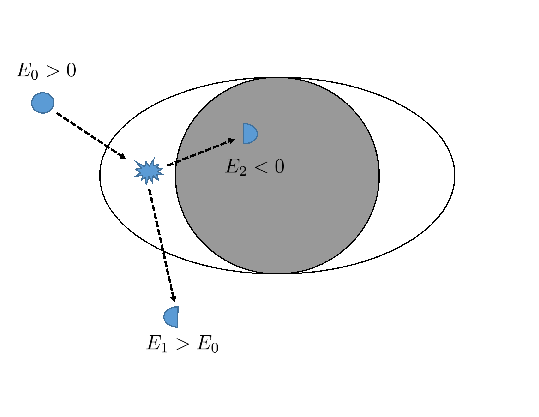
\includegraphics[width=\linewidth]{penrose_process.png}
	\caption{The Penrose Process. Source: \textcite{brito2020}.}
	\label{fig:penrose_process}
\end{figure}

Zde přichází nejjednodušší myšlenka generátoru založeného na Penroseově procesu, takzvaného Penroseova stroje. Je popsán v \textcite{misner1973}. Představme si jednoduchý mechanismus Penroseova stroje v podobě soustavy vozíků vhazujících odpadky do ČD (viz obrázek (\ref{fig:penrose_machine})). Předpokládejme, že máme železniční plošinu, která se pohybuje po kruhové dráze kolem rotujícího ČD a nachází se v jeho ergosféře. Na plošině jsou vozíky s nákladem, které se mohou oddělit a část nákladu vyhodit dovnitř HU. Když se vozík přiblíží k HU, rozdělí se na dvě části: jeden vozík vyvrhne trosky dovnitř HU a druhý je od ní odstrčen v opačném směru. V ergosféře existuje oblast, kde částice může mít zápornou energii vzhledem k pozorovateli v nekonečnu. To znamená, že pokud úlomky narazí do ČD se zápornou energií, ČD ztratí část své rotační energie. Druhý vozík při tom získá dodatečnou energii a zrychlí se, takže opustí ergosféru s větší rychlostí, než měl původně. V důsledku toho pozorovatel v nekonečnu uvidí, že soustava získala dodatečnou energii v důsledku rotace ČD, aniž by jí byla dodána energie z vnějšího zdroje. Je tedy možné periodicky vypouštět vozíky s nákladem, vhazovat část jejich hmotnosti dovnitř HU a získávat tak další a další urychlené vozíky.

\begin{figure} % Single column figure
	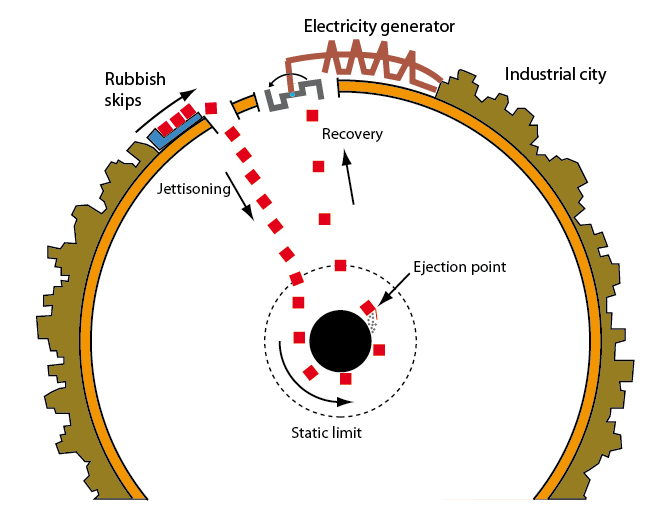
\includegraphics[width=\linewidth]{penrose_machine.jpg}
	\caption{Industrial extraction of energy from a black hole. Source: \href{https://blogs.futura-sciences.com/e-luminet/2016/01/16/warped-science-interstellar-46-time-dilation-penrose-process/}{The Warped Science of Interstellar (4/6) : Time dilation and Penrose process}.}
	\label{fig:penrose_machine}
\end{figure}

%------------------------------------------------

\section{Diskuze}

Využití ČD jako zdroje energie představuje pro vyspělé civilizace fascinující možnost. Teoretické modely, včetně Penroseova procesu, naznačují, že rotující ČD mohou poskytovat značné energetické výnosy. Zatímco experimentální vytvoření ČD na Zemi zůstává nedosažitelné, jejich astrofyzikální protějšky nabízejí přirozené prostředí pro získávání energie. Jednou z hlavních výzev je efektivní zachycení a přeměna získané energie do využitelné formy bez nadměrných energetických ztrát.

Navíc konstrukce struktur, jako jsou Dysonovy sféry kolem ČD, představuje značnou technickou a materiálovou výzvu. Diskuse se rovněž dotýká důsledků takových energetických systémů pro mezihvězdnou expanzi, zejména ve světle potenciálních omezení vyplývajících z termodynamiky a kvantových efektů. Tato studie nakonec zdůrazňuje potřebu dalšího výzkumu fyziky ČD a jejích technologických aplikací, jakož i širší důsledky pro detekci vyspělých mimozemských civilizací prostřednictvím jejich energetických stop.

%----------------------------------------------------------------------------------------
%	 REFERENCES
%----------------------------------------------------------------------------------------

\printbibliography % Output the bibliography
%----------------------------------------------------------------------------------------

\end{document}
